\mychapter{validation}{Validation \& Experiments}

To validate how CloudML addresses the requirements from~\citechap{requirements},
a topology of three nodes~(\citefig{threenodes}) is provisioned.
The experiment aims at validating that a topology can be expressed as CloudML lexical templates.
The experiment should also prove that nodes are provisioned through \emph{cloudml-engine}
to two different providers, without changing the templates.
The validation will provision on two different providers, \myac{AWS} and Rackspace.

This topology is the same as Alice used for her second scenario in \citesec{meta-model}.
The setup is sufficient to do a full deployment of the \emph{BankManager} application.

\paragraph{Template.}
\begin{figure}
  \begin{center}
    \begin{minted}[mathescape,
                   linenos,
                   numbersep=5pt,
                   gobble=2,
                   frame=lines,
                   framesep=2mm]{json}
{
  "name": "test",
  "loadBalancer": {
    "name": "test",
    "protocol": "http",
    "loadBalancerPort": 80,
    "instancePort": 80
  },
  "nodes": [{   
    "name": "front-end1",
    "minCores": 2,
    "minRam": 1000
  }, {   
    "name": "front-end2",
    "minCores": 2,
    "minRam": 1000
  }, {   
    "name": "back-end",
    "minDisk": 2000
  }]
}
    \end{minted}
  \end{center}
  \caption{Template for validation.}
  \label{list:validation-threenodes}
\end{figure}


\begin{figure}[tb]
  \begin{center}
    account.json:
    \begin{minted}[mathescape,
                   linenos,
                   numbersep=5pt,
                   frame=lines,
                   framesep=2mm]{json}
{
  "provider": "aws-ec2", 
  "identity": "...",
  "credential": "..."
}
    \end{minted}
  \end{center}
  \caption{Account used for validation, \emph{JavaScript Object Notation}~(JSON).}
  \label{list:validation-account}
\end{figure}



The implementation uses \myac{JSON} to define templates as a human readable serialization mechanism.
The lexical representation of \citefig{threenodes} can be seen in \citelist{validation-threenodes}.
There are a total of three files:
\begin{description}
  \item[account.json.]
    Expressed in \citelist{validation-account}, used to authenticate against a provider.
    In \citelist{validation-threenodes} \texttt{aws-ec2} is set as \texttt{provider},
    \ie nodes are created on \myac{AWS}.
    The two other properties, \texttt{identity} and \texttt{credential} are used for authentication.
    For \myac{AWS} that means \emph{Access Key ID} and \emph{Secret Access Key},
    while for Rackspace this is \emph{username} and \emph{API Key}.
  \item[front-ends.json.]
    Defines front-end nodes of the topology.
    Each node have specific attributes regarding their tasks, similar to Alice's scenario,
    but as an additional precaution the \texttt{front-end} nodes have increased \myac{RAM}.
  \item[back-end.json.]
    Defines the back-end node of the topology.
    Even though this is a separate file it is a part of the same topology,
    and it is provisioned beside the front-end nodes.
\end{description}
%All nodes in the first template are bound to the load balancer~(\texttt{loadBalancer})
%defined within the template.
The topology is split into two templates to support a load balancer,
as every node within a template will be bound to a given load balancer.
%The load balancer is yet introduced as it is not supported, more about the load balancer in~\citechap{perspectives}.
%since the \texttt{back-end} node should not be bound to the load balancer.
The splitting is by design, as a \texttt{template} is not directly bound to a topology,
and is also why \texttt{build} accept a list of templates.
The whole text represents the \texttt{Template} and consequently 
``\texttt{nodes}'' is a list of \texttt{Node} from the model.
The \myac{JSON} is textual which makes it \emph{shareable} as files.
Once such a file is created it can be reused (\emph{reproducibility}) 
on any supported provider (\emph{multi-cloud}).
These benefits match the requirement \citereq{lexical-template}.

\paragraph{Client.}
\begin{figure}[tb]
  \begin{center}
    \begin{minted}[mathescape,
                   linenos,
                   numbersep=5pt,
                   frame=lines,
                   framesep=2mm]{scala}

import no.sintef.cloudml.engine.Engine
import no.sintef.cloudml.repository.domain._
  ...
val runtimeInstances = Engine(account, templates)
println("Got " + runtimeInstances.size + " nodes")
runtimeInstances.foreach(ri => {
  println("Adding listener to: " + ri.instance.name + 
    " (" + ri.status + ")")
  ri.addListener( (event) =>  {
    event match {
      case Event.Property => 
      case Event.Status => 
        println("Status changed for " + ri.instance.name + 
          ": " + ri.stat
        if (ri.status ==  Status.Started) {
          println("Node " + ri.instance.name + 
            " is now running: " + ri)
        }
    }
  }
})
    \end{minted}
  \end{center}
  \caption{Code snippets of client used for validation (Scala).}
  \label{list:validation-client}
\end{figure}



Validation is done through a \myac{CLI}-based client application written in Scala.
Code snippets of this client is expressed in \citelist{validation-client}.
The snippets does not contain code to read the files, this is left out to save space.
File reading is done through Scala with \texttt{io.Source.fromFile(\emph{filename}).mkString}.
What files to read is specified through command line arguments,
where the first argument corresponds to account information,
and subsequent arguments are template files.

To initialize provisioning the client calls 
\texttt{val runtimeInstances = Engine(account, templates)}.
According to the meta model~(\citefig{meta-model}) this is the \texttt{build}-operation.
The name ``\emph{build}'' is a general term, while the usage in \citelist{validation-client}
is a Scala-specific pattern.
What Scala does here is syntactic sugar, when the client calls \texttt{Engine()},
Scala converts this into \texttt{Engine.apply()}.
This operation is overridden in \texttt{Engine}, so the logic is controlled by \emph{cloudml-engine}.

After receiving a list of \texttt{RuntimeInstances} the client runs through these 
objects and attach ``listeners''.
These listeners works according to the observer pattern,
when a property is added or the instance changes status,
a callback is made to the client.
This callback is done asynchronous through actor model.
Both of these solutions solves the requirement \citereq{m@rt}.

\paragraph{Provisioning.}
\begin{figure}
  \begin{center}
    \begin{minted}[numbersep=5pt,
                   frame=lines,
                   framesep=2mm]{text}
mvn scala:run 
  -DaddArgs="account.json|front-ends.json|back-end.json"

[INFO] Scanning for projects...
[INFO]
   ...
Got 3 nodes
Adding listener to: front-end1 (Building)
Adding listener to: front-end2 (Configuring)
Adding listener to: back-end (Configuring)
Status changed for front-end1: Starting
Status changed for front-end1: Started
Node front-end1 is now running: 
  RuntimeInstance(Instance(front-end1,2,2,0,))
Status changed for front-end2: Building
Status changed for front-end2: Starting
Status changed for front-end2: Started
Node front-end2 is now running: 
  RuntimeInstance(Instance(front-end2,2,2,0,))
Status changed for back-end: Building
Status changed for back-end: Starting
Status changed for back-end: Started
Node back-end is now running: 
  RuntimeInstance(Instance(back-end,0,1,500,))
    \end{minted}
  \end{center}
  \caption{Output from running validation client.}
  \label{list:validation-output}
\end{figure}



The client is built using Maven, to execute it the \texttt{scala:run}-\emph{goal} is called.
The three files,
\begin{ii}
  \iitem account.json,
  \iitem front-ends.json and
  \iitem back-end.json,
\end{ii}
are passed in as arguments to the client.
The final command looks like this:
\texttt{mvn scala:run \\ -DaddArgs="account.json|front-ends.json|back-end.json"}.
Output from executing this command is expressed in \citelist{validation-output}.
Some of the output is chunked away to save space.
The text in \citelist{validation-output} correlates to the 
client expressed in~\citelist{validation-client},
\ie information about status changes and when each node is successfully provisioned.

The output is identical for both \myac{AWS} and Rackspace.

\paragraph{After provisioning.}
\begin{figure}[tb]
  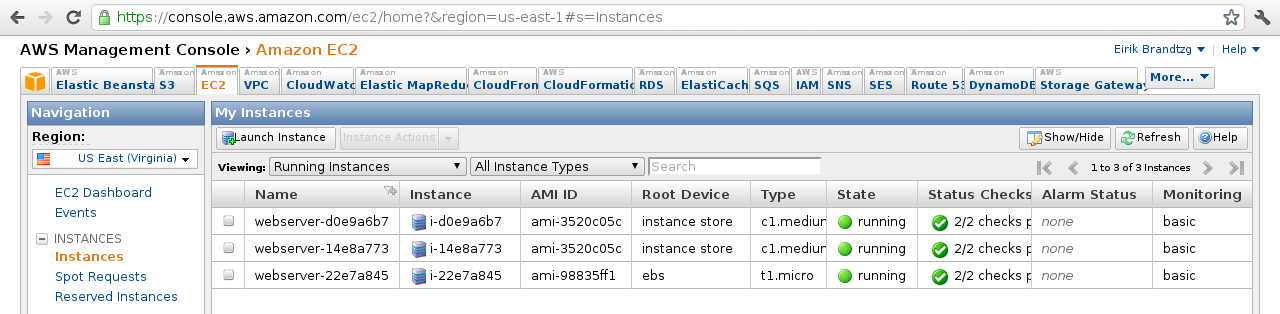
\includegraphics[width=\linewidth]{imgs/aws-console.png}
  \caption{Screenshot of \myac{AWS} console after validation provisioning.}
  \label{fig:validation-aws}
\end{figure}

\begin{figure}[tb]
  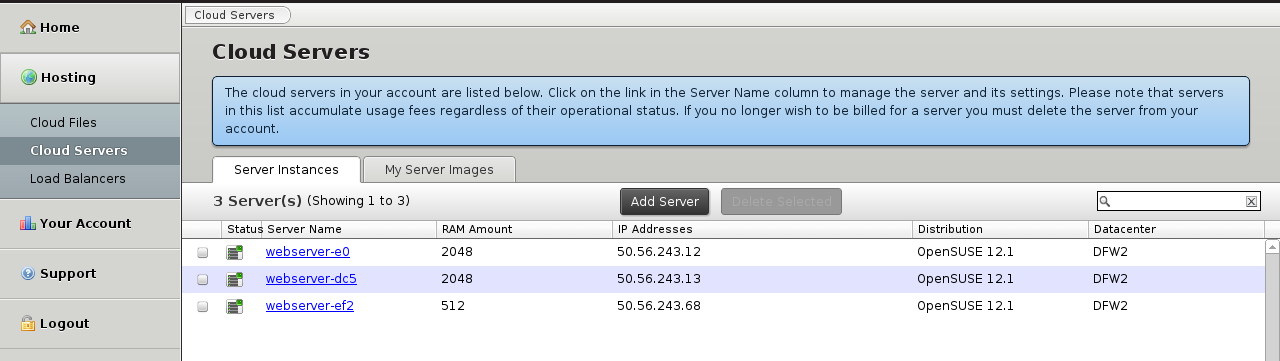
\includegraphics[width=\linewidth]{imgs/rackspace-console.png}
  \caption{Screenshot of Rackspace console after provisioning.}
  \label{fig:validation-rackspace}
\end{figure}


To validate the experiment screenshots of the cloud console of each provider are made.

The screenshot of \myac{AWS} console~(\citefig{validation-aws}) shows that three nodes
are successfully provisioned.
Two of the nodes is of the type \texttt{c1.medium} which corresponds to the template configuration.
The last node is a \texttt{t1.micro}, \ie this is the \texttt{back-end} node.
This is further emphasized by the fact that it uses \myac{EBS} as \texttt{Root device},
to achieve additional disk space.

Screenshot of Rackspace~(\citefig{validation-rackspace}) indicate similar consistencies,
\eg \texttt{RAM Amount} for each node, which corresponds with the template.
